% Concise GRAPE-style version. Tables/figures auto-generated from results/ (never hand-edit).
% Prose register: paper-writing skill craft_reference.md (plain words, ~21-word sentences,
% claim-first, active voice, no em-dashes).
\documentclass[10pt]{article}
\usepackage[margin=1in]{geometry}
\usepackage{amsmath,amsthm}
\usepackage{newtxtext,newtxmath}
\usepackage{graphicx,booktabs}
\usepackage[numbers,sort&compress]{natbib}
\usepackage[colorlinks,citecolor=blue,linkcolor=blue,urlcolor=blue]{hyperref}
\usepackage{microtype}
\newtheorem{proposition}{Proposition}
\newtheorem{definition}{Definition}
\newcommand{\T}{T}

\title{CGA: Conditioning as Group Action}
\author{Richard Bao\\ \texttt{richardbao419@gmail.com}}
\date{}

\begin{document}
\maketitle

\begin{abstract}
Networks are usually conditioned by scaling features (FiLM) or by generating weights
(hypernetworks). Both learn what each condition does. Neither learns what two conditions do
\emph{together} unless training data shows them together. We condition differently: rotate the
features, and make the rotation angles a linear function of the condition. Rotations add, so
combined conditions produce combined effects automatically. The network handles condition
combinations it never saw. We call the framework \textbf{CGA} (Conditioning as Group Action):
the condition enters the operator linearly in an abelian Lie algebra,
$\T(c)=P\exp(\mathrm{A}(Wc))P^{\top}$, so $\T(c_1{+}c_2)=\T(c_1)\T(c_2)$ holds exactly for any
weights. Known methods drop out as special cases: a diagonal algebra gives a compositional
variant of FiLM, and the rotation algebra with scalar position gives RoPE. Our version costs
$1.11\times$ FiLM's conditioning compute and uses fewer parameters than every baseline. We test
it under a pre-registered protocol: success margins, statistical tests, and data splits were
fixed and committed before each run. Across five transformation suites (synthetic operators,
dSprites, 3D~Shapes), CGA has the lowest error on never-trained condition combinations, with
complete seed separation ($p{=}9.1{\times}10^{-5}$, $N{=}10$). It extrapolates to longer
combinations than training ever contained. Replacing its linear map with an MLP, holding
everything else fixed, raises error by up to $4.3{\times}10^{4}$. The most expressive baselines
generalize worst. Three pre-registered gates also returned negatives, and we report them: a
$1.46\times$ fit penalty on rich scenes; a $7\times$ failure when the condition specifies image
content (a rotation moves information and cannot add it); and no advantage in world-model
rollouts, where the bottleneck is representation consistency, not operator composition. The
negatives tell practitioners exactly where the method stops working. They also specify a
successor, which we built and tested under two further pre-registered gates: \textbf{Complex
FiLM} treats each feature pair as a complex number, with an expressive magnitude (FiLM's content
channel) and a linear phase (our composition channel). It beats FiLM by 36\% on unseen change
combinations and matches FiLM on content generation (0.97$\times$ its error) in the same
diffusion setting where the pure rotation failed. One operator now covers both roles at
FiLM-class cost.
\end{abstract}

\section{The framework}

Let $x\in\mathbb{R}^d$ be features and $c\in\mathbb{R}^k$ a condition. FiLM
\citep{perez2018film} computes $y=\gamma(c)\odot x+\beta(c)$. AdaLN in DiT blocks
\citep{peebles2023dit} is its normalized form. Hypernetworks emit full weights $W(c)$
\citep{ha2017hypernetworks}. All of these are instances of
\begin{equation}
y=\T(c)\,x+\beta(c),
\label{eq:family}
\end{equation}
and they differ only in where the per-sample operator $\T(c)$ comes from.

\begin{definition}[Compositional conditioner]
$\T:\mathbb{R}^k\!\to\!\mathrm{GL}(d)$ is \emph{compositional} if it is a homomorphism from
$(\mathbb{R}^k,+)$: $\T(c_1{+}c_2)=\T(c_1)\,\T(c_2)$ and $\T(0)=I$.
\end{definition}

\begin{proposition}[Exact composition by construction]
\label{prop:main}
Let $\mathfrak{a}$ be an abelian subalgebra of $\mathfrak{gl}(d)$, $\mathrm{A}:\mathbb{R}^m\!\to\!
\mathfrak{a}$ linear, $W\in\mathbb{R}^{m\times k}$, and $P$ orthogonal. Then
$\T(c)=P\exp(\mathrm{A}(Wc))\,P^{\top}$ is a compositional conditioner for every $W,P$. If
$\mathfrak{a}$ is skew-symmetric, $\T(c)$ is orthogonal.
\end{proposition}
\begin{proof}
$\exp(X)\exp(Y)=\exp(X{+}Y)$ for commuting $X,Y$; $\mathrm{A}\circ W$ is linear; conjugation
preserves products; $\exp(0)=I$.
\end{proof}

The point is simple. Composition is usually a behavior the network must learn from data. Here it
is a property of the parametrization. It holds at initialization, during training, and far
outside the training distribution. Training only decides \emph{which} directions the condition
rotates and \emph{how fast}.

\paragraph{Special cases.} Choices of $(\mathfrak{a}, c, P)$ recover deployed mechanisms:

\begin{center}
\small
\begin{tabular}{llll}
\toprule
$\mathfrak{a}$ & condition & $P$ & recovered mechanism \\
\midrule
$\mathrm{diag}(\mathbb{R}^d)$ & $c$ & $I$ & \emph{exponential FiLM}: $y=e^{Wc}\odot x$ (compositional) \\
$\mathfrak{so}(2)^{d/2}$ & $c=n$ (scalar position) & $I$ & RoPE \citep{su2021rope} \\
$\mathfrak{so}(2)^{d/2}$ & $c=n$, learned planes & learned & multiplicative GRAPE \citep{grape2025} \\
$\mathfrak{so}(2)^{d/2}$ & general $c\in\mathbb{R}^k$ & structured & \textbf{this work} (FiLM's role) \\
$\mathrm{diag} \times \mathfrak{so}(2)^{d/2}$ & general $c$ & canonical & \textbf{Complex FiLM} (the successor; \S\ref{sec:exp}) \\
\bottomrule
\end{tabular}
\end{center}

Standard FiLM reaches the same diagonal operators through an MLP head $\gamma(c)$. The operators
match; the composition law is missing. Section~\ref{sec:exp} shows the missing law is exactly
what fails on unseen combinations: an ablation with the same operators, the same basis, and more
compute loses by up to $4.3\times10^4$ once its map from condition to operator is an MLP. The
PEFT literature (LoRA, OFT, BOFT, HRA, Group-and-Shuffle
\citep{hu2022lora,qiu2023oft,liu2024boft,yuan2024hra,gorbunov2024gs}) uses these operator
families to fine-tune \emph{weights}, one fixed transform per task. CGA uses them in FiLM's
role: a new operator per sample, applied to activations, where the composition question lives.

\paragraph{Cost.}
With $\mathfrak{a}=\mathfrak{so}(2)^{d/2}$, $\exp$ is a closed-form planar rotation: $3d$ FLOPs,
no matrix exponential. The basis $P$ is the whole budget question. A dense learned $P$ costs
$4d^2$ FLOPs per sample, which is $1.52\times$ FiLM's entire conditioning path at $d{=}128$. Two
fixes work. First, a structured orthogonal $P$ (five block-diagonal Cayley layers with fixed
shuffles, following Group-and-Shuffle) brings the total to $1.11\times$ FiLM. This $P$ has
4{,}800 parameters against the 8{,}128 dimensions of $\mathrm{SO}(128)$, and that is enough: it
only needs to find the planes the condition acts on. Second, inside a transformer no explicit
$P$ is needed at all. The dense projections next to the rotation learn the basis, which is how
RoPE works. The operator equals the identity at initialization and at $c{=}0$, and every
singular value is 1. Unit tests pin all three properties.

\section{Experiments}
\label{sec:exp}

\paragraph{Protocol.} Every suite is pre-registered. We fixed the success margins, the tests
($N{=}10$ seeds, one-sided Mann--Whitney $p\le0.01$, Cliff's $|\delta|\ge0.474$), and the data
splits before each run, and committed them to version control. Each test split is read once. All
arms share one backbone and one training recipe. A shared counter enforces the budget: our
conditioning path stays within $1.20\times$ FiLM's FLOPs and $1.05\times$ the smallest
hypernetwork baseline's parameters. Baselines may be bigger, and reach $48\times$ our parameter
count. We report every verdict, including the negatives. Baselines: FiLM, conditional LayerNorm,
Concat-MLP, a dense hypernetwork $I{+}\Delta W(c)$, a dynamic low-rank map
$I{+}A(c)B(c)^{\top}$, and an MLP-head ablation of our own method.

\paragraph{Suites.} \textbf{S1/S2 (synthetic):} learn $y=M(c)x$, where $c$ selects a combination
of 8 rotation primitives. S2 hides the primitives behind a random basis and also tests all 56
never-trained \emph{triples}. \textbf{S3/S3b (dSprites) and S4 (3D~Shapes):} image
transformation. Encode a real image, apply $\T(\Delta)$ to the latent for a factor change
$\Delta$, decode, and score pixel error against the true transformed image. OOD means
never-trained \emph{types} of two-factor changes. S3b and S4 add a categorical shape factor.
\textbf{S5 (content):} a small diffusion transformer generates dSprites images from full factor
specifications; held-out combinations have unique ground-truth images, so generation error is
objective. \textbf{S6 (rollouts):} a world model applies the conditioning arm recurrently, one
action per step; we test unseen action-type pairs and rollouts of length 10 and 20 after
training on length 3. \textbf{S7 (the successor, two gates):} Complex FiLM, magnitude from
FiLM's MLP head and phase linear in the condition, rerun through the S3 transformation suite
and the S5 content suite.

\begin{table}[t]
\centering
\caption{Error on never-trained condition combinations (mean over 10 seeds). CGA is lowest in
every column, with complete seed separation against the strongest hypernetwork baseline
($p{=}9.1{\times}10^{-5}$, $\delta{=}{-}1.0$). S1--S3b pass the full pre-registered gate; S4
fails a separate fit criterion (text).}
\label{tab:main}
% AUTO-GENERATED by gen_tables.py — do not edit
\begin{tabular}{lcccccc}
\toprule
Conditioner & S1 & S2 & S3 & S3b & S4 & S7 \\
\midrule
FiLM & $1.3\,(0.1)\!\times\!10^{-2}$ & $1.6\,(0.04)\!\times\!10^{-2}$ & $3.0\,(0.2)\!\times\!10^{-3}$ & $5.9\,(0.2)\!\times\!10^{-3}$ & $4.5\,(1.0)\!\times\!10^{-3}$ & $3.1\,(0.2)\!\times\!10^{-3}$ \\
Concat-MLP & $1.5\,(0.3)\!\times\!10^{-2}$ & $1.1\,(0.4)\!\times\!10^{-2}$ & $2.9\,(0.1)\!\times\!10^{-3}$ & $6.3\,(0.2)\!\times\!10^{-3}$ & $5.4\,(5.2)\!\times\!10^{-3}$ & -- \\
Cond-LN & $2.4\,(0.1)\!\times\!10^{-2}$ & $2.7\,(0.05)\!\times\!10^{-2}$ & $3.2\,(0.2)\!\times\!10^{-3}$ & $6.1\,(0.3)\!\times\!10^{-3}$ & $8.6\,(13.1)\!\times\!10^{-3}$ & -- \\
Hypernetwork & $1.9\,(0.3)\!\times\!10^{-3}$ & $3.4\,(0.9)\!\times\!10^{-3}$ & $3.8\,(0.3)\!\times\!10^{-3}$ & $7.0\,(0.4)\!\times\!10^{-3}$ & $9.3\,(2.3)\!\times\!10^{-3}$ & $3.8\,(0.2)\!\times\!10^{-3}$ \\
Dyn.\ low-rank & $5.7\,(0.5)\!\times\!10^{-3}$ & $6.1\,(0.4)\!\times\!10^{-3}$ & $5.1\,(0.9)\!\times\!10^{-3}$ & $8.1\,(0.4)\!\times\!10^{-3}$ & $2.0\,(0.4)\!\times\!10^{-2}$ & -- \\
MLP-head (abl.) & -- & $1.1\,(0.2)\!\times\!10^{-3}$ & $2.7\,(0.2)\!\times\!10^{-3}$ & $5.0\,(0.2)\!\times\!10^{-3}$ & $3.3\,(0.8)\!\times\!10^{-3}$ & -- \\
Complex FiLM (lin.) & -- & -- & -- & -- & -- & $2.0\,(0.1)\!\times\!10^{-3}$ \\
\textbf{Complex FiLM} & -- & -- & -- & -- & -- & $2.0\,(0.2)\!\times\!10^{-3}$ \\
\textbf{Lie (ours)} & $7.4\,(2.0)\!\times\!10^{-4}$ & $3.3\,(2.2)\!\times\!10^{-8}$ & $1.8\,(0.1)\!\times\!10^{-3}$ & $4.0\,(0.1)\!\times\!10^{-3}$ & $1.2\,(0.2)\!\times\!10^{-3}$ & $1.8\,(0.1)\!\times\!10^{-3}$ \\
\bottomrule
\end{tabular}
% gate margins: S1: 62\% vs.\ hypernet ($p=9e-5$); S2: 100\% vs.\ hypernet ($p=9e-5$); S3: 54\% vs.\ hypernet ($p=9e-5$); S3b: 43\% vs.\ hypernet ($p=9e-5$); S4: 87\% vs.\ hypernet ($p=9e-5$); S7: 0\% vs.\ ? ($p=0e+00$)

\end{table}

\begin{figure}[t]
\centering
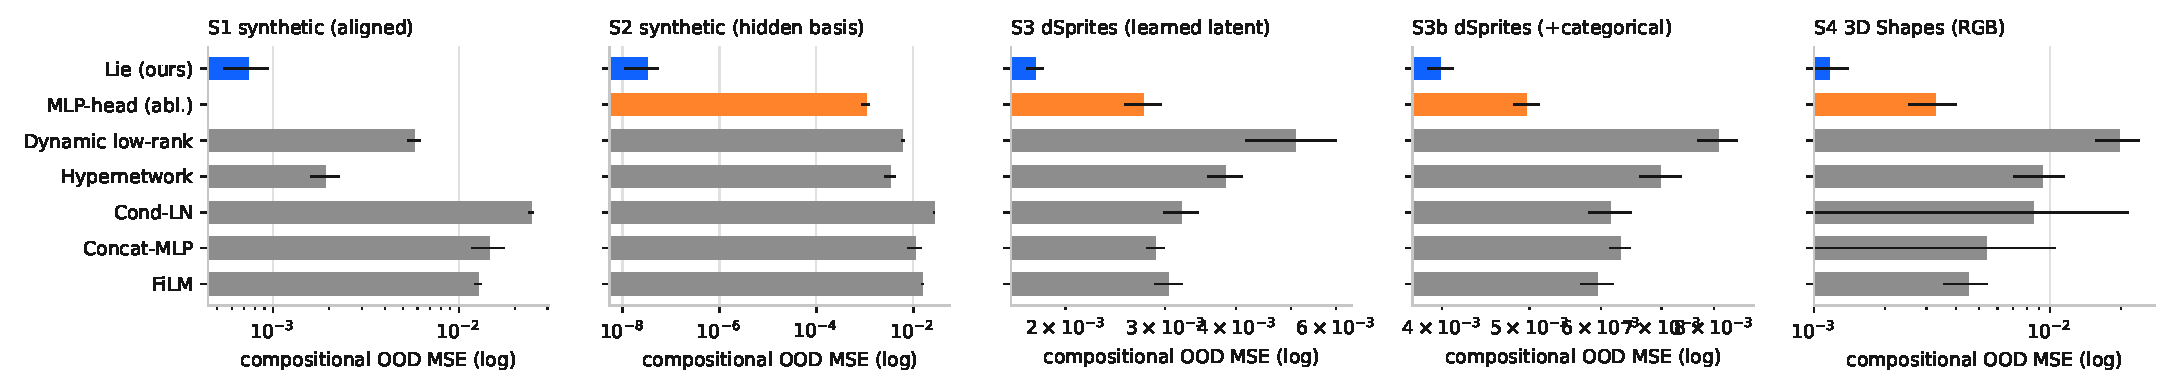
\includegraphics[width=\textwidth]{figs/f1_ood_all_stages.pdf}
\caption{Error on unseen condition combinations, by conditioner (log scale; blue = CGA, orange =
MLP-head ablation).}
\label{fig:main}
\end{figure}

\paragraph{Findings.}
\textbf{(1) When conditions form a group, composition is solved.} On S2, CGA reaches
$3.3{\times}10^{-8}$ error on unseen pairs and $5.3{\times}10^{-8}$ on never-trained triples.
The best baseline sits five orders of magnitude higher, and every baseline gets worse as
combinations get longer. CGA does not. Its learned angles match the true generators to
$2{\times}10^{-4}$ rad, so the operator is directly readable.
\textbf{(2) The advantage survives learned representations.} On dSprites, every arm fits the
training distribution equally well, so the comparison isolates composition. CGA's error grows
$1.25\times$ from training to unseen combinations ($1.63\times$ with the categorical factor).
Every baseline grows $2.1$--$3.3\times$. CGA beats the strongest baseline by $53.8\%$ ($42.9\%$)
at $39\times$ fewer conditioning FLOPs.
\textbf{(3) The linear map is the mechanism.} The ablation keeps the basis and the operator
family, spends more compute, and swaps only the linear map for an MLP. It loses by
$4.3{\times}10^{4}\times$ on synthetic triples and $1.55\times$ on dSprites.
\textbf{(4) More capacity makes it worse.} The two hypernetwork arms can express any operator.
They post the worst generalization gaps on images ($2.7$--$26\times$). Their capacity goes into
memorizing the training combinations.
\textbf{(5) Three registered negatives.} On 3D~Shapes, CGA has the best OOD numbers ($87.5\%$
margin) but fits the training distribution $1.46\times$ worse than the best memorizer, which
trips our no-regression gate. In the content suite, rotation conditioning fails ($0.31$ vs.\
film's $0.04$), and the ablation fails identically: a rotation moves information around and
cannot add any, so it cannot carry ``generate this image.'' In the rollout suite, every arm
compounds error at the same rate, and the mildly contractive low-rank arm degrades least. Each
step of a rollout adds a small mismatch between the predicted and true latent. A contraction
shrinks that mismatch at every step; an isometry carries it forever. Exact operator composition
cannot repair an inconsistent representation.

\section{Practical guidance: when to use this}
\label{sec:practical}

Three rules for practitioners, from the eight suites.

\textbf{Use phase conditioning when your conditions are changes that combine.} Edit deltas,
attribute offsets, pose or camera adjustments, applied once. The cost matches FiLM
($1.11\times$ FLOPs, fewer parameters), training-distribution quality matches, and behavior on
never-trained combinations is $43\%$ to $10^5\times$ better. FiLM's failure on new combinations
is silent: nothing in training warns you. The guarantee removes that failure class.

\textbf{For conditions that say what to generate, use Complex FiLM or keep FiLM.} Pure
rotation conditioning fails there ($7\times$ worse; our registered negative). Complex FiLM
matches FiLM on content ($0.97\times$) while keeping the composition wins, so it is the
candidate drop-in at our evidence scale; plain FiLM remains the conservative choice.

\textbf{In rollouts, pair an isometric operator with a consistency loss.} Without that loss,
all conditioners compounded error at the same rate. With it, the rotation operator's rollout
error stays flat where FiLM's grows $4.5\times$ and a hypernetwork's $10\times$: train the
transition to satisfy $\T(a)z_s \approx z_{s+1}$ and the isometry stops carrying old errors
forward because there are none to carry.

All evidence comes from controlled $64{\times}64$ benchmarks with known factors. Nothing here is
validated at production scale. The transformer variant costs less than FiLM's marginal class
path, so where the first rule applies, trying the swap is cheap.

\section{Discussion}

CGA does for conditioning what RoPE did for position: it moves composition from a behavior the
network must learn into a law the parametrization guarantees. Four boundaries are measured.
Categorical factors shrink the advantage. Rich scenes make orthogonality pay a fit penalty.
Content specification defeats a transformation channel. Rollouts are limited by representation
consistency, which no operator guarantee repairs. The first three pointed at one successor design, the algebra torus $\times$ diagonal, and S7
validated it: Complex FiLM carries content with its magnitude and composition with its phase.
The fourth boundary falls to a consistency objective on the representation: with it, the
isometric operator gives flat rollouts where every baseline drifts. Related work has learned group actions on latents for world models
\citep{quessard2020,caselles2019}; CGA differs by living in FiLM's role under a matched budget,
with composition holding by construction rather than by training objective.

\paragraph{Reproducibility.} Every suite is pre-registered, and every number in this paper
regenerates from committed logs. Unit tests pin the operator invariants and the budget counters.
The repository discloses all amendments and one accounting erratum.

\begin{thebibliography}{9}
\bibitem[Perez et al.(2018)]{perez2018film} E.~Perez et al. FiLM: Visual reasoning with a general
conditioning layer. \emph{AAAI}, 2018.
\bibitem[Peebles and Xie(2023)]{peebles2023dit} W.~Peebles, S.~Xie. Scalable diffusion models
with transformers. \emph{ICCV}, 2023.
\bibitem[Ha et al.(2017)]{ha2017hypernetworks} D.~Ha, A.~Dai, Q.~Le. Hypernetworks. \emph{ICLR}, 2017.
\bibitem[Su et al.(2021)]{su2021rope} J.~Su et al. RoFormer: Enhanced transformer with rotary
position embedding. \emph{arXiv:2104.09864}, 2021.
\bibitem[GRAPE(2026)]{grape2025} Anonymous. Group representational position encoding.
\emph{ICLR}, 2026. arXiv:2512.07805.
\bibitem[Hu et al.(2022)]{hu2022lora} E.~Hu et al. LoRA. \emph{ICLR}, 2022.
\bibitem[Qiu et al.(2023)]{qiu2023oft} Z.~Qiu et al. Orthogonal finetuning. \emph{NeurIPS}, 2023.
\bibitem[Liu et al.(2024)]{liu2024boft} W.~Liu et al. BOFT. \emph{ICLR}, 2024.
\bibitem[Yuan et al.(2024)]{yuan2024hra} S.~Yuan et al. Householder reflection adaptation.
\emph{NeurIPS}, 2024.
\bibitem[Gorbunov et al.(2024)]{gorbunov2024gs} M.~Gorbunov et al. Group and shuffle: Efficient
structured orthogonal parametrization. \emph{NeurIPS}, 2024.
\bibitem[Quessard et al.(2020)]{quessard2020} R.~Quessard, T.~Barrett, W.~Clements. Learning
disentangled representations and group structure of dynamical environments. \emph{NeurIPS}, 2020.
\bibitem[Caselles-Dupr\'e et al.(2019)]{caselles2019} H.~Caselles-Dupr\'e, M.~Garcia-Ortiz,
D.~Filliat. Symmetry-based disentangled representation learning requires interaction with
environments. \emph{NeurIPS}, 2019.
\end{thebibliography}

\end{document}
